
%%%%%%%%%%%%%%%%%%%%%%%%%%%%%%%%%%%%%%%%%%%%%%%%%%%%%%%%%%%%%%%%%%%%%%%%%
%           Capítulo 2: MARCO TEÓRICO - REVISIÓN DE LITERATURA
%%%%%%%%%%%%%%%%%%%%%%%%%%%%%%%%%%%%%%%%%%%%%%%%%%%%%%%%%%%%%%%%%%%%%%%%%

\chapter{Marco teórico}
\section{Fuentes de voltaje en aceleradores de partículas}

Después de la construcción del primer acelerador, en la misma década de los
30, se inventaron otros tipos de aceleradores tales como el ciclotrón, los
aceleradores lineales y los aceleradores tipo Van de Graaff. Debido a que los
primeros aceleradores de partículas se construyeron con el fin de estudiar
experimentalmente la estructura del núcleo atómico, por medio de colisiones las que
podían originar transmutaciones o reacciones nucleares, fue la razón por lo que al
hablar de un acelerador se asociaba automáticamente con un laboratorio de física
nuclear. La importancia de estos instrumentos de física nuclear es similar a la del
telescopio en astronomía o al microscopio en bacteriología.\\

 Actualmente el uso de
los aceleradores se ha extendido a otras áreas de investigación básica como la
física atómica el mundo de los electrones y en las partículas elementales. Los
aceleradores en medicina se usan tanto en los departamentos de radiología, para
destruir tumores malignos, como para producir radioisótopos que se utilizan en el
diagnóstico de enfermedades (medicina nuclear). El uso de los aceleradores en
aplicaciones tecnológicas es muy variado y el más conocido es en las industria de
los semiconductores y de la núcleo-electrónica, las cuales se usan un tipo especial
de aceleradores conocidos como implantadores con los que es posible producir
los chips electrónicos, circuitos integrados, etc\\

Los aceleradores son instrumentos relativamente complejos y su diseño y
construcción requiere de alta tecnología e intervienen muchos campos de la
ingeniería. Una forma de clasificar los aceleradores es por la energía de los
proyectiles y los de alta energía o superaceleradorores están instalados, por
ejemplo en algunos laboratorios nacionales de los EUA, tal como, en Los Alamos,
BrookHaven, FermiLab y en Europa en el CERN. \\

Las instalaciones de estos superaceleradores son impresionantes por su gran
tamaño y los cientos de toneladas de materiales que se requirieron para su
construcción. Por ejemplo, el acelerador en el FermiLab es circular y tiene un radio de 1 Km. Sin embargo los conceptos sobre los principios de operación de los
superaceleradores y de los pequeños aceleradores son los mismos y son simples y
se describen a continuación.\\

Un diagrama simplificado de un acelerador de partículas se muestra
esquemáticamente en la figura 2.1 y cuyos elementos básicos son:\\

1) Fuente de voltaje\\
2) Fuente de iones (en el esquema es un filamento)\\
3) Electrodos.

\begin{figure}[H]
\centering
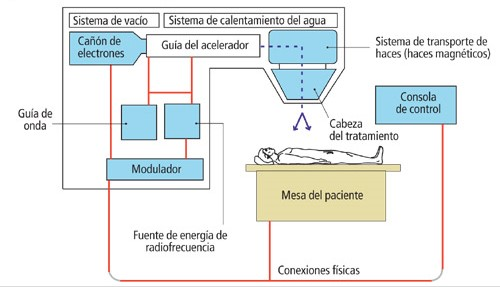
\includegraphics[width=12cm]{capitulo2/figs/acelerador.png}
\caption{Diagrama esquemático de las componentes principales de un acelerador de
partículas.}
\end{figure}

El principio de funcionamiento del cualquier tipo de acelerador, se basa en la
interacción de los campos eléctricos producidos por fuentes de voltaje sobre la
carga eléctrica de las partículas generadas en la fuente de iones y esta es la razón por la que no se pueden acelerar partículas neutras.\\

Otras partes importantes asociadas a un acelerador son equipos periféricos
tales como: sistemas de vacío, líneas de transporte de haz, cámaras de
experimentación, etc. Un tubo de rayos X y el cinescopio de una TV doméstica según la definición
anterior son aceleradores de partículas, sin embargo, en la práctica no se les refiere con este nombre.\\

Como se sabe, las unidades que se usan para la energía en física son los julios
y/o ergios. Sin embargo, para cuantificar la energía de los proyectiles acelerados se acostumbra usar unidades de electrón-volt (eV) o sus múltiples: el keV= 1 000 eV, el $MeV= 1 000 000 eV$, el TeV= $10^{12} eV$, etc. El uso de estas unidades de energía
es debido a la relación simple de la ecuación anterior, en la cual la energía es
numéricamente igual al voltaje. De acuerdo con la ecuación anterior, una energía
de 1 eV es el cambio de energía cinética que experimenta una partícula con carga
en valor absoluto igual a la del electrón, después de pasar por una diferencia de
potencial de un volt. \cite{acelerado}

\newpage
\section{Calculo de capacidad de corriente en pistas de circuitos impresos}



Antes de comenzar con la fabricación de un diseño de PCBs se debe de considerar el tamaño de pistas necesarios para el manejo de corrientes para cada circuito desarrollado, por esa razón mediante un análisis se debe avanzar en el diseño.\\

En la actualidad los desarrolladores llevan a reducir el ancho de las pistas y espacios, debido a que se desarrollan componentes cada vez más pequeños y sistemas igualmente más compactos, esto obliga a adaptarse a estos nuevos requerimientos.\\

Para encontrar una solución a esta eventualidad es necesario recurrir a estudios en estos temas que nos permita acercarnos al límite y para ello debemos de considerar todos los parámetros que influyan en nuestro sistema, obteniendo así resultados más precisos. En nuestro caso nos basaremos en los gráficos publicados en el IPC2152 \cite{IPC 2152} ``Standard for Determining Current Carry Capacity in Printed Board Design'' en 2009, este estándar es ampliamente utilizado en muchos proyectos que requieran este tipo de análisis. \\  

Para el correcto entendimiento de los procesos que influyen en las pistas por el paso de la corriente debemos de recordar que el paso de la corriente por un conductor produce en este una caída de potencial que esta gobernada por la ley de OHM (R=V/I), esta caída de potencial se disipa en forma de calor por el efecto Joule $Q=I^{2}Rt$. En nuestro el conductor es nuestra pista, su resistencia depende de varios factores, pero lo principal es su sección (ancho x espesor) y su longitud. El efecto térmico es en realidad el que nos interesa conocer al momento del dimensionamiento de la PCB. Por esta razón, para poder calcular una capacidad de transporte de corriente, hay que analizarlo en términos de incremento de temperatura. Fijando como un incremento maxico admisible.\\

Existen algunos parámetros que se deben de considerar importantes de conocer, ya que los mismos alteran o modifican el comportamiento termico de la pista, afectando de manera significativa, los mas importantes son:\\

\begin{itemize}
\item Corriente eléctrica que circula.
\item Tipo de material base.
\item Calculo de corriente de pistas.
\item Sección de la pista.
\item Espesor del laminado de cobre.
\item Espesor de la placa.
\item Presencia de planos de tierra o grandes áreas de cobre.
\item Ambiente de aplicación (gabinete, forzadores de aire, vacío, etc.)
\end{itemize}

Considerar todos estos parámetros en un modelo es bastante complicado, tanto que, en sí, el estándar fue fijado por medio de ensayos y presentando los resultados en forma de curvas. Mediante estos datos empíricos se hace una aproximación que se acerque al límite que deseamos, tomando en cuenta que es importante sobredimensionar dichos límites. \\

El cálculo que se realiza se basa en el fijado de una variación máxima de temperaturas admisibles. La variación térmica se define como un aumento de temperatura por encima de la temperatura inicial que experimenta el conductor. \\
Para el cálculo se requieren los gráficos ya antes mencionados que son dos. El primer grafico es una de las tres entradas y se trata de una serie de curvas que corresponden a los incrementos de temperatura desde diez a cien grados centígrados. En el eje de las ordenadas se grafica la corriente máxima en amperes y en el de las abscisas obtenemos la sección de la pista en milésimas de pulgada cuadrada. El segundo grafico tiene de igual manera tres entradas y en esta se centra en el espesor del cobre, adoptando los valores típicos en los que se fabrican las PCBs, llegando desde 0.5 hasta 3 Oz/ft2.\\

Los cálculos necesarios son sencillos y claros de realizar, para ello necesitaremos los siguientes datos:\\

\begin{itemize} 
\item Corriente máxima a soportar.
\item Incremento máximo de temperatura admisible.
\item Espesor de cobre del material utilizado.
\end{itemize}
Utilizando el valor de corriente nos ubicamos en la figura 2.1 por el eje de las ordenadas y proyectamos el valor en forma paralela al eje de las abscisas hasta interceptar la curva que corresponde a la temperatura máxima admisible, luego en la figura 2.2 tomamos el punto en las ordenadas hasta obtener el valor de las absisas que le corresponde. Ese valor es el valor de la sección cuadrada que debe de tener la pista.

\begin{figure}[H]
\centering
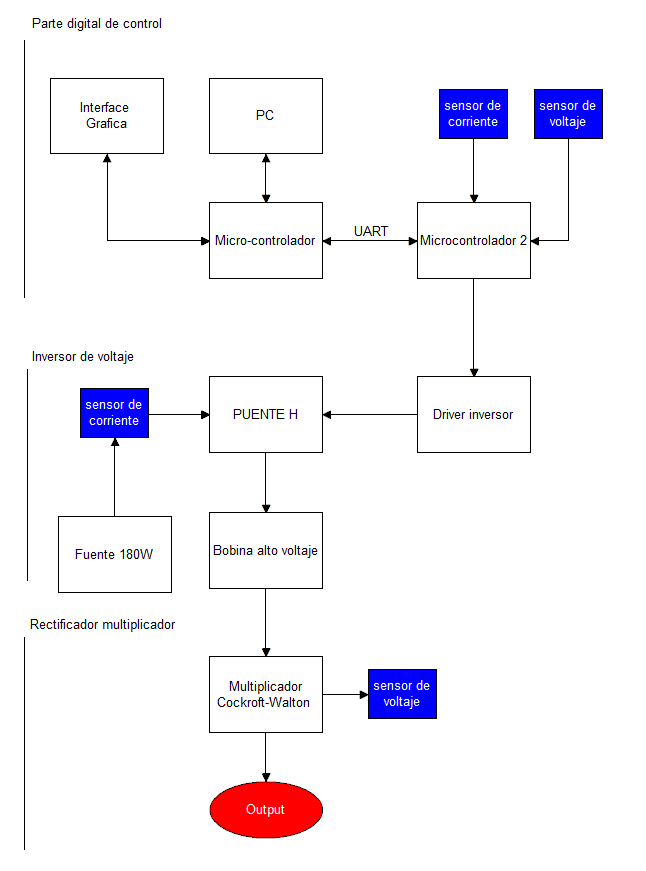
\includegraphics[width=12cm]{capitulo2/figs/figura1.png}
\caption{Calculo de ancho de pistas 1}
\end{figure}

\begin{figure}[H]
\centering
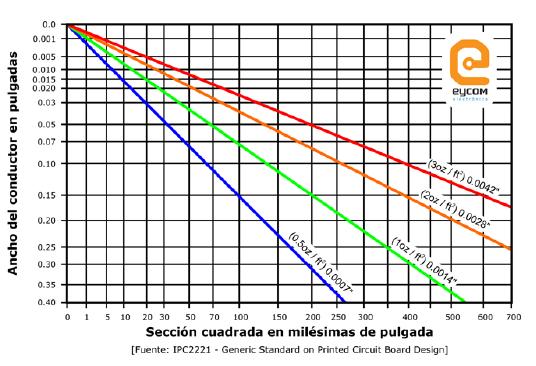
\includegraphics[width=12cm]{capitulo2/figs/figura2.png}
\caption{Calculo de ancho de pistas 1}
\end{figure}

\newpage
\section{Fuente de voltaje lineal}
Es común en proyectos de electrónica no especializados la utilización de diferentes tipos de fuentes de voltaje, entre las que se encuentran fuentes lineales, conmutadas, boost o tipo buck y los problemas que puede causar la falta de atención en este punto tan crucial puede afectan los resultados finales de un proyecto. Es por ello que se necesita conocer los principios fundamentales que reinan a este tipo de sistemas que gobernaran el comportamiento de nuestro proyecto al nivel mas básico.\\

La fuente de voltaje lineal consiste en un sistema sencillo y estructurado, el cual se diseña en diferentes configuraciones en cada modulo a partir del tipo de carga que requiere el proyecto. Para ello podemos observar en la figura 2.5 de manera ilustrativa el orden de la estructura básica de una fuente lineal.

\begin{figure}[H]
 \centering
 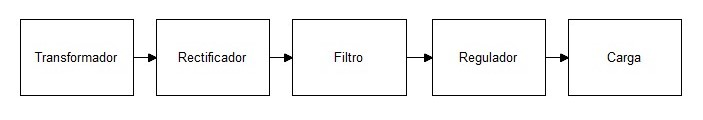
\includegraphics[width=12cm]{capitulo2/figs/fuentelineal.jpg}
 \caption{Estructura fuente lineal}
 \end{figure}
 
 De manera independiente podemos analizar cada aspecto presentado en la imagen, el cual, de uno en uno se va realizando un análisis para definir los valores y topologias que satisfacen las necesidades requeridas. Tomando en cuenta lo mencionado podemos comenzar a definir las ecuaciones y modelos existentes.
 \newpage

\subsection{Etapa de transformador monofasico}

Esta etapa consta básicamente de un transformador que esta formado por un bobinado primario y uno o varios bobinados secundario, que tiene como función principal
convertir la energía eléctrica alterna de la red, en energía alterna de otro nivel de voltaje, por medio de la acción de un campo magnético. Ademas provee una aislación galvánica entre la entrada y la salida.\\

Los transformadores son máquinas estáticas con dos devanados, de corriente alterna enrollados sobre un núcleo magnético. El devanado por donde entra energía al transformador se denomina primario y el devanado por donde sale energía hacia las cargas que son alimentadas por el transformador se denomina secundario. El devanado primario tiene $N_{1}$ espiras y el secundario tiene $N_{2}$ espiras. El circuito magnético de esta máquina lo constituye un núcleo magnético sin entrehierros, el cual no está realizado con hierro macizo sino con chapas de acero silicio apiladas y aisladas entre sí. De esta manera se reducen las pérdidas magnéticas del transformador.\\

Al inducir una corriente sobre cualquiera de los dos devanados se genera un flujo alterno en el núcleo magnético. Este flujo magnético se describe mediante la Ley de Faraday y produce una fuerza electromotriz que da lugar a una tensión $V_{2}$ en los bornes de dicho devanado.\\

Normalmente, para un transformador reductor o un transformador elevador tienen dos devanados que se denominan de alta tension y de baja tensión, siendo bobina primaria y bobina secundaria respectivamente. Un mismo transformador puede alimentarse por el lado A.T. y funcionar como transformador reductor o alimentarse por el lado de B.T. y actuar como un transformador elevador.

\begin{figure}[H]
\centering
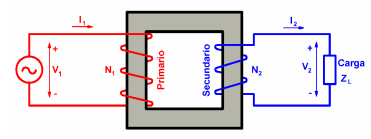
\includegraphics[width=9cm]{capitulo3/figs/trans.png}
\caption{ Principio de funcionamiento de un transformador monofásico.}
\end{figure}

En la figura 2.5 podemos observar los símbolos mas comunes que representan al transformador. 

\begin{figure}[H]
\centering
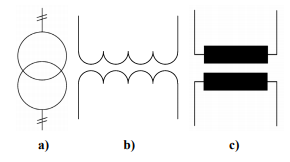
\includegraphics[width=7cm]{capitulo3/figs/simbolos.png}
\caption{ Simbologia de un transformador monofásico.}
\end{figure}

Ahora podemos definir los valores asignados o nominales para el diseño de un transformador.\\

Las \textbf{tensiones asignadas o nominales} ($V_{1}$, $V_{2}$) son aquellas para las que se ha diseñado el transformador, estas tenciones son proporcionales al numero de espiras ($N_{1}$,$N_{2}$) de cada devanado.\\

La \textbf{potencia asignada o nominal} ($S_{N}$) la cual permite un funcionamiento sin calentamientos peligrosos en su funcionamiento normal. Cabe mencionar que los dos devanados siempre tendrán la misma potencia asignada.\\

Las \textbf{corrientes nominales o asignadas} ($I_{1N}$,$I_{2N}$) se obtienen a partir de las tensiones asignadas y de la potencia asignada. Así, en un transformador monofásico se tiene que:

\begin{equation}\label{eq:ej}
S_{N}=V_{1N}*I_{1N}=V_{2N}*I_{2N}
\end{equation}
La \textbf{relación de transformación} (m) es el cociente entre las tensiones asignadas del primario y del secundario: 

\begin{equation}\label{eq:ej}
m=\dfrac{V_{1N}}{V_{2N}}
\end{equation}

Estudiando superficialmente los aspectos de construcción de un transformador, mediante estas ecuaciones podemos comenzar con la construcción y diseño. Debemos de considerar las potencias necesarias para nuestro proyecto y mediante ellas calcular el ancho del cobre y el tamaño del entre-hierro.\cite{transformador}
\newpage

\subsection{Rectificador monofasico de onda completa}

El circuito rectificador de onda completa enera una señal de corriente directa (D.C.) a partir de una señal de corriente alterna
(A.C.) con todos los semiciclos de la señal, invirtiendo todos los semiciclos de una misma polaridad, para convertirlos a la otra. 

\begin{figure}[H]
\centering
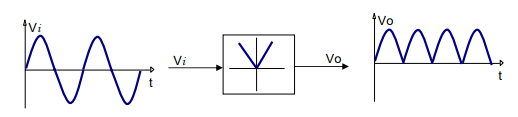
\includegraphics[width=12cm]{capitulo3/figs/puente.png}
\caption{ Simbologia de un transformador monofásico.}
\end{figure}

Para calcular el voltaje de D.C. que obtendremos podemos utilizar la siguiente ecuación\cite{rectificador}


\begin{equation}\label{eq:ej}
V_{cd}=2*0.636V_{m}
\end{equation}

\newpage
\subsection{Filtros}
El voltaje de CA por lo general se conecta a un transformador, el cual lo reduce al nivel de salida de DC deseado. Un rectificador de diodos proporciona entonces un voltaje rectificado de onda completa, el cual en principio se pasa por un filtro de capacitor sencillo para producir un voltaje de DC. El cual en todos los casos presenta un voltaje de riso o variación de voltaje de CA.\\

Para calcular el voltaje de riso podemos utilizar un multimetro con capacidad de medir voltaje en CA (TRUE RMS) y el voltaje de DC. El voltimetro de cd leerá solo el nivel promedio. El medidor de ca (RMS) leerá solo el valor RMS del componente de ca del voltaje de salida. Entonces, definimos el riso como:\\

\begin{equation}
r=\frac{voltaje\:  de\:  riso\:  (rms)}{voltaje\:  de\:  DC}=V_{cd}\cdot 100\%
\end{equation}

\begin{figure}[H]
\centering
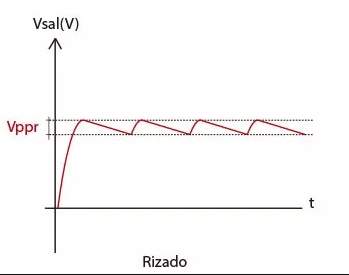
\includegraphics[width=7cm]{capitulo3/figs/risado.png}
\caption{ Forma de onda de un voltaje filtrado que muestra voltajes de dc y de rizo.}
\end{figure}

\begin{figure}[H]
\centering
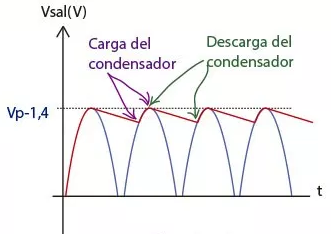
\includegraphics[width=7cm]{capitulo3/figs/filtro.png}
\caption{ Forma de onda de un voltaje filtrado que muestra voltajes de dc y de rizo.}
\end{figure}

Para nuestro caso utilizaremos un filtro de capacitor. Se conecta un capacitor en la salida del rectificador y se obtiene un voltaje de dc a través del capacitor como se muestra en la figura 2.7 y 2.8. Podemos calcular el \textbf{voltaje del riso} que obtendremos mediante la ecuación:

\begin{equation}
V_{r}(rms)=\dfrac{I_{cd}}{4\sqrt{3}fC}=\dfrac{2.4V_{cd}}{R_{L}C}
\end{equation}

Con la ecuación 2.4 podemos intuir y definir la expresion para el \textbf{rizo} de la forma de onda de salida de un rectificador de onda completa y el circuito de capacitor de filtrado:

\begin{equation}
r=\dfrac{V_{r}I_{cd}}{CV_{cd}}*100\%=\dfrac{2.4}{R_{L}C}
\end{equation}
\newpage
\subsection{Regulador}

Un factor de importancia en una fuente de alimentación es la cantidad de cambios de voltaje de salida de cd a lo largo de la operación de un circuito. El voltaje provisto a la salida en la condición sin carga (sin que demande corriente de la fuente) se reduce cuando se extrae corriente de carga de la fuente. La cantidad que el voltaje de DC cambia entre las condiciones sin carga y con carga la describe un factor llamado regulación de voltaje, para una fuente ideal la regulación de voltaje seria del 0\%. Entonces podemos definir la regulacion de voltaje como:
 

$$Regulaci\acute{o}n\:de\: voltaje = \dfrac{Voltaje\: sin \:carga \:-\: Voltaje\: con\: carga}{voltaje\: con\: carga}$$
\begin{equation} 
 \%V.R. = \dfrac{V_{NL}-V_{FL}}{V_{FL}}*100\%
\end{equation}





\newpage

\section{Inversores de voltaje}

Los convertidores DC a AC se conocen como inversores. La función de un inversor es cambiar un voltaje de entrada de DC a un voltaje simétrico de salida de AC de magnitud y frecuencia deseada. 
Los inversores se pueden clasificar ampliamente en dos tipos: inversores monofasicos e inversores trifasicos. Cada tipo puede usar dispositivos de encendido y apagado controlados, por ejemplo transistor de unión bipolar (BJT), transistor de efecto de campo metal-óxido-semiconductor(MOSFET),transistor bipolar de puerta aislada (IGBT), etc. Por lo general estos inversores utilizan señales de control de PWM para producir un voltaje de salida de CA.

Existen diferentes tipos de inversores, un inversor se conoce como inversor alimentado por voltaje (VFI) si el voltaje de entrada permanece constante; inversor alimentado por corriente (CFI) si el voltaje de entrada permanece constante, e inversor enlazado en cd variable si el voltaje de entrada es controlable. Si al voltaje o a la corriente de salida del inversor se le hace pasar a través de cero al crear un circuito LC resonante, a este tipo de inversores se le conoce como inversor de pulso resonante, y tiene vastas aplicaciones en la electrónica de potencia. \\

\subsection{Parametros de desempeño de un inversor}

El voltaje de entrada a un inversor es de DC y el voltaje de salida de AC. Idealmente la salida debe de ser una onda sinusoidal pura, pero contiene armónicos o rizos como se muestra en l figura 2.7. El inversor consume corriente de la fuente de entrada de DC solo cuando se conecta la carga al sistema, afectando la calidad de la señal de salida, es por ello que una medición variara conforme se conecte una carga diferente. Por lo común la calidad de un inversor se evalúa en función de los siguientes parámetros de desempeño:\\

La potencia de salida esta dada por \begin{equation}
P_{ca}=I_{0}V_{0}COS\theta
\end{equation}
\begin{equation}
P_{ca}= I_{0}^{2}R
\end{equation}

Donde $V_{0}$ e $I_{0}$ son el voltaje y corriente rms de la carga, $\theta$ es en angulo de la impedancia de la carga y R es la resistencia de la carga.\\

La potencia de entrada de ca del inversor es:\\

\begin{equation}
P_{S}=I_{S}V_{S}
\end{equation}

donde $V_{S}$ e $I_{S}$ son el voltaje y la corriente promedio de entrada.\\

El contenido de riso rms de la corriente de entrada es:

\begin{equation}
I_{R}=\sqrt{I_{I}^{2}-I_{S}^{2}}
\end{equation}

donde $I_{I}$ e $I_{S}$ son los valores rms y promedio de la corriente de suministro de cd.
El factor de rizo de la corriente de entrada es: 

\begin{equation}
RF_{s}=\dfrac{I_{r}}{I_{s}}
\end{equation}

La eficiencia de potencia, la cual es la relación de la potencia de salida a la potencia de entrada, dependerá de las perdidas por conmutación, que a su vez dependen de la frecuencia de conmutación del inversor.\\

Factor armonico del n-ésimo armonico (H$F_{n}$). El factor armonico (del n-ésimo armonico) que mide la contibuciónarmonca individual, se define como \begin{equation}
HF_{n}=\dfrac{V_{on}}{V_{o1}}, \: para\; n>1
\end{equation}

donde $V_{O1}$ es el valor rms del componente fundamental y $V_{ob}$ es el valor rms del n-ésimo componente armónico.\\

Distorsion armonica total (THD). La distorsion armonica total, que mide la cercaia en cuanto a forma de onda y su componente fundamental, se define como: \begin{equation}
THD=\dfrac{1}{V_{O1}}\left( \sum_{n=2,3,...}^{\infty }V_{on}^{2}\right)
\end{equation}

Factor de distorsión (DF).
 
\newpage
\section{Multiplicador de voltaje Cockcroft-Walton}
Cockroft-Walton es un multiplicador de voltaje desarrollado para fines nucleares \cite{CERN}. Este generador consiste en un arreglo en cascada de diodos y capacitores para generar alto voltaje en corriente directa (CD) mediante una entrada de de voltaje en corriente alterna (CA). El sistema Cockoft-Walton es usado principalmente en aceleradores de partículas, pero también en sistemas láser, tubos CRT, LCDs, fuentes de voltaje y sistemas de rayos X. Podemos observar el sistema en cuestión en la figura 1.  

\begin{figure}[H]
\centering
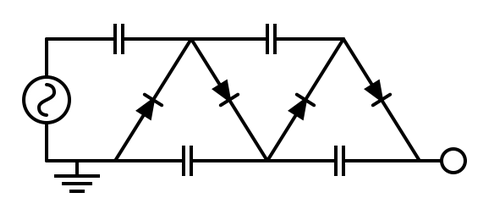
\includegraphics[width=9cm]{capitulo2/figs/circ.png}
\caption{ Circuito en cascada Cockroft-walton de media onda.}
\end{figure}
El sistema multiplicador es bastante sencillo pero existen algunos temas imprescindibles los cuales tenemos que estudiar a profundidad, ya que el funcionamiento fundamental de un capacitor es la carga y descarga del mismo, es por ello que los parámetros del componente deben de ser calculados metódicamente.

\begin{figure}[H]
\centering
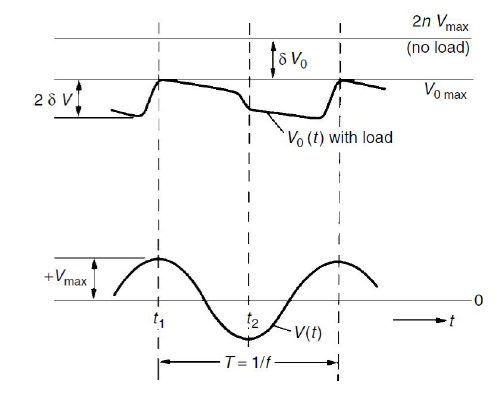
\includegraphics[width=9cm]{capitulo2/figs/riso.png}
\caption{ Reproducción del voltaje $V_{o}$ y el riso $\delta$V en la carga del circuito.}
\end{figure}

\begin{equation}
\delta V=\frac{i}{fC}\frac{n(n+1)}{4}
\end{equation}

\begin{equation}
V\approx 2nV-\frac{2n^{3}}{3fC}
\end{equation}

Es por ello que mediante un análisis matemático debemos de hacer el calculo de la respectiva $\delta$ del mismo.\\
No solamente la calidad de la salida depende de lo antes mencionado, ya que, para un correcto funcionamiento necesitamos realizar un sistema de entrada estable y constante. De aquí el siguiente estudio.
\newpage
\section{Transformadores de alto voltaje.}

Los transformadores de alto voltaje son utilizados ampliamente en sistemas tanto industriales, médicos como de investigación. Una de estas tantas aplicaciones son los sistemas de ignición, ya que, por el alto voltaje que tenemos en el secundario se producen arcos eléctricos en situaciones controladas, que pueden servir para ignición de combustoleos. En el área de la medicina también se utiliza de manera importante en sistemas de generación de ozono, rayos X, entre tantas otras cosas mas.  \\

\subsection{Sistemas de encendido.}

Cuando las líneas de fuerza de un campo magnético son
interrumpidas por un conductor (alambre) en movimiento, se crea en éste
una corriente eléctrica. Este fenómeno es conocido con el nombre de
inducción electromagnética.\\

\begin{figure}[H]
\centering
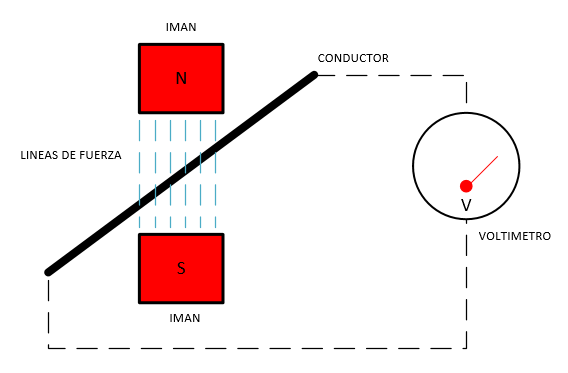
\includegraphics[width=12cm]{capitulo3/figs/induc.png}
\caption{ Inducción electromagnética.}
\end{figure}

``Este fenómeno se manifiesta de igual manera ya sea que se
mueva el campo magnético, el conductor o ambos. Obviamente, el voltaje
inducido en el conductor variará según la intensidad del campo magnético
pero también tendrá que ver la velocidad con que se mueva el conductor o el campo magnético. Asimismo, si enrollamos el conductor formando una
bobina y con ella interrumpimos las líneas de fuerza, el voltaje en el
conductor se multiplicará tantas veces como vueltas del alambre pasen a
través del campo.''\\

\begin{figure}[H]
\centering
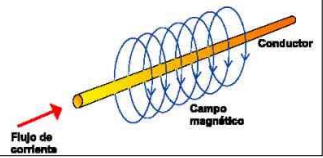
\includegraphics[width=12cm]{capitulo3/figs/trans2.png}
\caption{ Inducción electromagnética 2.}
\end{figure}

En la figura 2.14 se aprecia la estructura básica de un transformador
de encendido. La corriente de la batería (12V) fluye por el arrollamiento
primario y crea un potente campo magnético que se concentra en el
núcleo y envuelve al arrollamiento secundario. AI interrumpirse la corriente
por medio del sistema electrónico de encendido, el campo se colapsa
hacia el núcleo férrico atravesando en su camino al arrollamiento
secundario donde se induce un elevado voltaje (35 000 V aprox.) Este
proceso de carga y descarga del transformador se repite tan rápido como
lo requiera el régimen del motor para el encendido de las bujías


\begin{figure}[H]
\centering
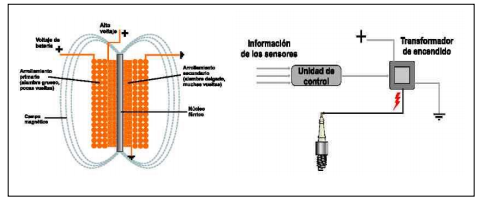
\includegraphics[width=12cm]{capitulo3/figs/trans3.png}
\caption{ Estructura básica transformador de encendido.}
\end{figure}

El encendido electrónico es un concepto muy amplio pues existen
tantos sistemas diferentes como recursos tecnológicos. Algunos sistemas
a base de transistores; otros con sistema Hall y algunos más que utilizan
un reluctor, todos realizan, a un nivel de alta tecnología, lo que el sistema
mecánico de platinos desempeñó durante muchos años para lograr el
mismo objetivo.\\

Sobre estas líneas se encuentra un esquema muy simplificado de
un sistema de encendido electrónico donde la Unidad de Control se
encarga de abrir y cerrar el circuito primario, con base en la información
que le Ilega de los sensores indicándole las condiciones de
funcionamiento del motor. \cite{ignicion}

\subsection{Generación de rayos X}

El sistema de funcionamiento de un generador de rayos X tiene un funcionamiento relativamente básico.  El equipo recibe electricidad desde la corriente domestica, esta corriente puede ser de 220 V a 440 V, es recibido por un transformador de baja tension que es reductor y que baja el voltaje a 5 o 10 v, lo cual va a producir incandescencia del filamento, generando liberación de electrones. Estos electrones son centralizados por la copa centralizadora de Molibdeno, y que se quedan ahí, en el filamento de tungsteno, esperando. \\

Cuando el equipo se dispara, con el cronorruptor, se activa el circuito de alta tensión que tiene un transformador amplificador, lo que genera un aumento de voltaje a 70Kv. Al ser tan grande la diferencia de potencial entre en ánodo y el cátodo va a generar una gran diferencia de potencial y los electrones salen disparados al ánodo. 

Los electrones se dirigen al ánodo y chocan contra una barra de tungsteno. Cuando se activa el circuito de baja tension, no se liberan los electrones; quedan en el filamento de tungsteno.\\

\begin{figure}[H]
\centering
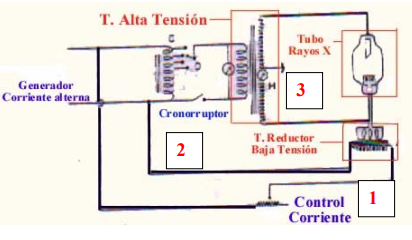
\includegraphics[width=12cm]{capitulo3/figs/rayos.png}
\caption{ Tubo de rayos x}
\end{figure}

Las aplicaciones de estos tubos de rayos x son bastas y han sido un gran avance tecnológico para la humanidad. La generación de rayos x mediante voltaje tiene sus pros y sus contras respecto a generación de rayos x por isotopos radiactivos, ya que los tubos de rayos x pueden ser apagados cuando el equipo no esta operando, en cambio el isotopo radiactivo estará permanentemente irradiando, perdiendo intensidad con el pasar del tiempo.  \\

